

En este capítulo se presenta la planificación del proyecto, abordando el alcance definido, los periodos de realización de tareas y los diversos ámbitos de gestión: temporal, de riesgos, de comunicaciones e información, y de partes interesadas. El objetivo de esta planificación es establecer una hoja de ruta estructurada que permita el cumplimiento de todos los objetivos del proyecto dentro de los plazos establecidos.

\section{Alcance}

Este proyecto aborda el desarrollo de un sistema basado en agentes LLM implementado sobre una solución software propia de LKS NEXT, con el propósito de investigar el comportamiento de diversas arquitecturas de agentes definidas en el capítulo \ref{ch:chap2} y evaluar su viabilidad para su futura incorporación en los procesos productivos de la empresa.

En dicho sistema, se implementarán diversas modalidades de interacción entre agentes especializados en fuentes de datos específicas, evaluando la eficacia de los distintos patrones de comunicación entre dichos componentes.

Cabe destacar que el alcance del proyecto no está definido en su totalidad, dada la complejidad de estimación inherente a su naturaleza exploratoria y al uso de tecnologías emergentes. Para mitigar riesgos en el desarrollo, se ha establecido un protocolo preventivo que contempla reuniones quincenales de seguimiento y control.

\subsection{Objetivos concretos del proyecto}

Para facilitar el logro del objetivo principal, se han identificado y definido los siguientes objetivos específicos que estructuran el avance progresivo del proyecto:

\begin{itemize}
  \item\textbf{Estudio de arquitecturas agénticas: }Realizar un análisis de las diversas arquitecturas de agentes, considerando distintas estrategias de interacción y mecanismos de acceso a fuentes de información.
  \item\textbf{Desarrollo de sistema de Onboarding: }Implementar las arquitecturas propuestas en un proyecto software corporativo, con el propósito de analizar su eficacia en la asistencia a nuevos integrantes durante su proceso de incorporación a la empresa.
  \item\textbf{Integración del Model Context Protocol: }Exploración de las características y beneficios que aporta la implementación del protocolo MCP, con el objetivo de realizar una valoración objetiva para su posible integración en el entorno profesional de la empresa.
  \item\textbf{Evaluación de agentes: }Desarrollar un sistema de evaluación para proporcionar métricas comparativas cuantificables sobre el rendimiento de los diferentes enfoques de agentes. 
  \item\textbf{Valoración de ajuste de agentes: }Analizar la relación coste-beneficio asociada al proceso de ajuste fino de modelos LLM para su aplicación en agentes concretos.
\end{itemize}

Adicionalmente, el proyecto contempla desarrollar el sistema de onboarding incorporando en la medida de lo posible en su base de conocimiento la metodología de trabajo implementada en la empresa. Mediante la adhesión a los estándares definidos en un entorno profesional real, se pretende garantizar que los resultados obtenidos constituyan un reflejo de la viabilidad de implementación y eficacia de proyectos similares en un sistema de explotación. 

\subsection{Requisitos}
Los requisitos del proyecto se detallan en profundidad en la sección ref:\textbf{siguiente capítulo}

\subsection{Fases del proyecto}
Tal y como se ha mencionado anteriormente, el alcance del proyecto no está completamente definido debido a su naturaleza exploratoria. Consecuentemente, se propone un ciclo de vida iterativo-incremental con iteraciones de aproximadamente dos semanas de duración, permitiendo una adaptación progresiva a los requisitos emergentes.

La primera iteración se centra en la captura de requisitos del proyecto, donde se explorará y definirá el alcance del sistema de agentes a desarrollar. Tras establecer estas bases, la segunda iteración abordará la implementación de un sistema de agentes mínimo que contenga la estructura general del sistema, proporcionando un marco operativo inicial.

Con este sistema mínimo implementado, la tercera iteración corresponderá al desarrollo de un mecanismo de evaluación, con el objetivo de establecer métricas que permitan mejorar el sistema en la cuarta iteración, donde se aplicarán las optimizaciones identificadas. La quinta iteración se dedicará a la implementación de arquitecturas de agentes exploratorias, evaluando su rendimiento mediante las métricas previamente establecidas.

Finalmente, la sexta iteración contemplará el ajuste fino de un modelo LLM para su integración en un agente específico del sistema, así como su evaluación contextualizada dentro del entorno funcional del proyecto.

Gracias a la implementación del ciclo de vida iterativo, se logra la consecución de los objetivos del proyecto de forma progresiva y estructurada. Este enfoque permite obtener retroalimentación constante por parte de los directores del proyecto durante cada iteración, facilitando así la posibilidad de reorientar la dirección del trabajo ante la aparición de posibles contratiempos.

\subsection{Descomposición de tareas}
La Estructura de Descomposición de Trabajo (EDT) del proyecto se ha creado considerando el ciclo de vida iterativo-incremental del proyecto. La figura \ref{fig:edt} ilustra un diagrama de esta. 

\begin{figure}[h]
  \centering
  \rotatebox{90}{%
    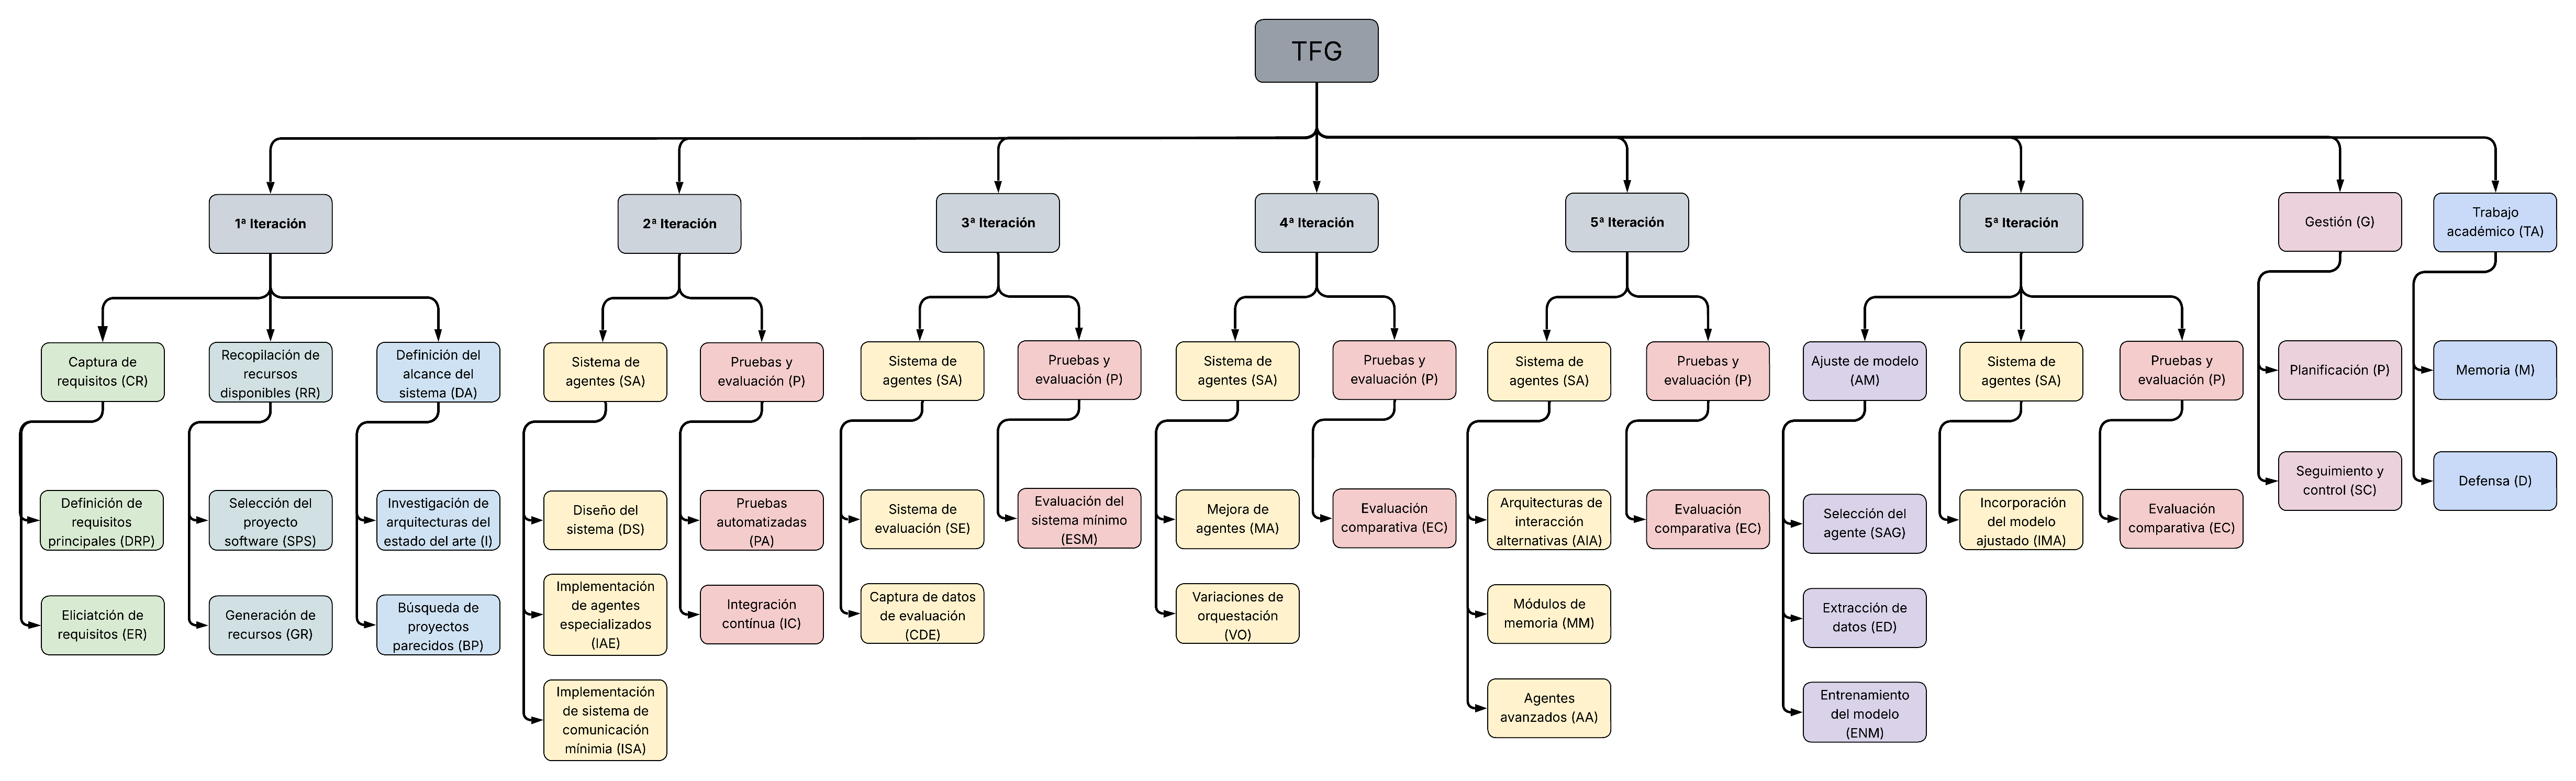
\includegraphics[scale=0.135]{figures/paquetes.png}%
  }
  \caption{Estructura de Descomposición de Trabajo (EDT) del proyecto}
  \label{fig:edt}
\end{figure}


Se divide en los siguientes paquetes:

\begin{itemize}
  \item\textbf{1ª iteración:}
    \begin{itemize}
      \item\textbf{Captura de requisitos (CR):} Actividades orientadas a la definición de los requisitos necesarios para el desarrollo del proyecto.
            \begin{itemize}
          \item\textbf{Definición de requisitos principales:} Identificación y documentación de los requisitos del proyecto, validados con los directores al inicio del mismo.
          \item\textbf{Elicitación de requisitos:} Recopilación de preguntas potenciales para el sistema desarrollado mediante cuestionario electrónico y análisis posterior de las respuestas.
        \end{itemize}
      \item\textbf{Recopilación de recursos disponibles (RR):} Actividades centradas en la selección y generación de recursos esenciales para el desarrollo.
        \begin{itemize}
          \item\textbf{Selección de proyecto software:} Identificación y documentación del proyecto software sobre el que se desarrollará el sistema.
          \item\textbf{Generación de recursos:} Elaboración de documentación complementaria para la implementación del sistema de agentes.
        \end{itemize}
      \item\textbf{Definición del alcance del sistema de agentes (DA):} Delimitación del alcance considerando implementaciones previas y trabajo académico existente.
    \begin{itemize}
          \item\textbf{Investigación de arquitecturas del estado del arte:} Análisis de las arquitecturas relevantes documentadas en la literatura académica.
          \item\textbf{Exploración de proyectos similares:} Estudio de implementaciones similares en proyectos software y procesos de Onboarding.
    \end{itemize}
      \end{itemize}
  \item\textbf{2ª iteración:}
    \begin{itemize}
      \item\textbf{Sistema de agentes (SA):} Actividades centradas en el diseño e implementación de un sistema de agentes LLM para asistencia en proyectos software.
        \begin{itemize}
          \item\textbf{Diseño del sistema:} Conceptualización e implementación básica de los módulos fundamentales del sistema.
          \item\textbf{Implementación de agentes especializados:} Desarrollo de agentes adaptados a las diversas fuentes de información disponibles.
          \item\textbf{Sistema de comunicación mínima:} Creación de un mecanismo básico de orquestación para los agentes implementados.
        \end{itemize}
      \item\textbf{Pruebas y evaluación (P):} Actividades destinadas a verificar y analizar el rendimiento de los módulos implementados.
        \begin{itemize}
        \item\textbf{Pruebas automatizadas:} Desarrollo de pruebas unitarias para algoritmos críticos de los agentes especializados.
        \item\textbf{Integración continua:} Implementación de un flujo de trabajo automatizado para la ejecución de pruebas unitarias.
      \end{itemize}
    \end{itemize}
  \item\textbf{3ª iteración:}
    \begin{itemize}
      \item\textbf{Sistema de agentes (SA):} Actividades centradas en el diseño e implementación de un sistema de agentes LLM para asistencia en proyectos software.
        \begin{itemize}
          \item\textbf{Sistema de evaluación:} Implementación de mecanismos de evaluación automática sobre el sistema mínimo.
          \item\textbf{Captura de datos de evaluación:} Anotación manual de ejemplos representativos para evaluar el rendimiento del sistema. 
        \end{itemize}
      \item\textbf{Pruebas y evaluación (P):} Actividades destinadas a verificar y analizar el rendimiento de los módulos implementados.
        \begin{itemize}
          \item\textbf{Evaluación del sistema mínimo: } Ejecución de evaluaciones automatizadas e identificación de elementos clave para mejoras posteriores.
        \end{itemize}
    \end{itemize}
  \item\textbf{4ª iteración:}
    \begin{itemize}
      \item\textbf{Sistema de agentes (SA):} Actividades centradas en el diseño, implementación y evaluación de un sistema de agentes LLM para asistencia en proyectos software.
        \begin{itemize}
          \item\textbf{Mejora de agentes:} Refinamiento de los agentes implementados para optimizar su rendimiento según las métricas establecidas.
          \item\textbf{Variaciones de orquestación:} Análisis e implementación de estrategias alternativas de orquestación. 
        \end{itemize}
      \item\textbf{Pruebas y evaluación (P):} Actividades destinadas a verificar y analizar el rendimiento de los módulos implementados.
        \begin{itemize}
          \item\textbf{Evaluación comparativa:} Ejecución de evaluaciones automatizadas y análisis comparativo respecto a la iteración anterior.
        \end{itemize}
    \end{itemize}
  \item\textbf{5ª iteración:}
    \begin{itemize}
      \item\textbf{Sistema de agentes (SA):} Actividades centradas en el diseño e implementación de un sistema de agentes LLM para asistencia en proyectos software.
        \begin{itemize}
          \item\textbf{Arquitecturas de interacción alternativas:} Implementación y evaluación de mecanismos adicionales de interacción entre agentes.
          \item\textbf{Módulos de memoria:} Integración de sistemas de memoria y evaluación de su impacto en el rendimiento global. 
          \item\textbf{Agentes avanzados:} Desarrollo de un agente con un proceso de ejecución extenso para el análisis del coste-beneficio.
        \end{itemize}
      \item\textbf{Pruebas y evaluación (P):} Actividades destinadas a verificar y analizar el rendimiento de los módulos implementados.
        \begin{itemize}
          \item\textbf{Evaluación comparativa: } Análisis del rendimiento de las nuevas características respecto al sistema precedente.
        \end{itemize}
    \end{itemize}
  \item\textbf{6ª iteración:}
    \begin{itemize}
      \item\textbf{Ajuste de modelo (AM):} Actividades orientadas al entrenamiento especializado de un modelo para un agente específico.
      \begin{itemize}
        \item\textbf{Selección del agente:} Identificación justificada del agente candidato para el ajuste del modelo.
        \item\textbf{Extracción de datos:} Recopilación automatizada de datos de entrenamiento mediante un modelo de alto rendimiento.
        \item\textbf{Entrenamiento del modelo:} Diseño y ejecución del ciclo de entrenamiento del modelo LLM seleccionado.
      \end{itemize}
      \item\textbf{Sistema de agentes (SA):} Actividades centradas en el diseño e implementación de un sistema de agentes LLM para asistencia en proyectos software.
        \begin{itemize}
          \item\textbf{Incorporación del modelo ajustado:} Desarrollo de adaptadores e integración del modelo en el sistema existente.
        \end{itemize}
      \item\textbf{Pruebas y evaluación (P):} Actividades destinadas a verificar y analizar el rendimiento de los módulos implementados.
        \begin{itemize}
          \item\textbf{Evaluación comparativa: } Análisis del rendimiento del sistema con el modelo ajustado frente a versiones anteriores.
        \end{itemize}
    \end{itemize}
  \item\textbf{Gestión (G):} 
    \begin{itemize}
      \item\textbf{Planificación (PL):} Establecimiento de directrices, objetivos y actividades para el desarrollo óptimo del proyecto.
      \item\textbf{Seguimiento y control (SC):} Monitorización periódica mediante reuniones bisemanales con los directores del proyecto.
    \end{itemize}
  \item\textbf{Trabajo académico (TA):}
    \begin{itemize}
      \item\textbf{Memoria (M):} Elaboración del documento académico que recoge todo el trabajo realizado.
      \item\textbf{Defensa (D):} Preparación de la presentación y defensa del proyecto ante el tribunal evaluador.
    \end{itemize}
\end{itemize}

\section{Periodos de realización de tareas e hitos}
En este apartado se detallan las dependencias entre las diferentes tareas, así como la estimación de duración y fechas de cada una de ellas.

\subsection{Dependencias entre tareas}
Las dependencias de los paquetes de trabajo del proyecto requieren una ejecución secuencial planificada. La figura \ref{fig:dependencias} ilustra dichas dependencias.

\begin{figure}[h]
  \centering
  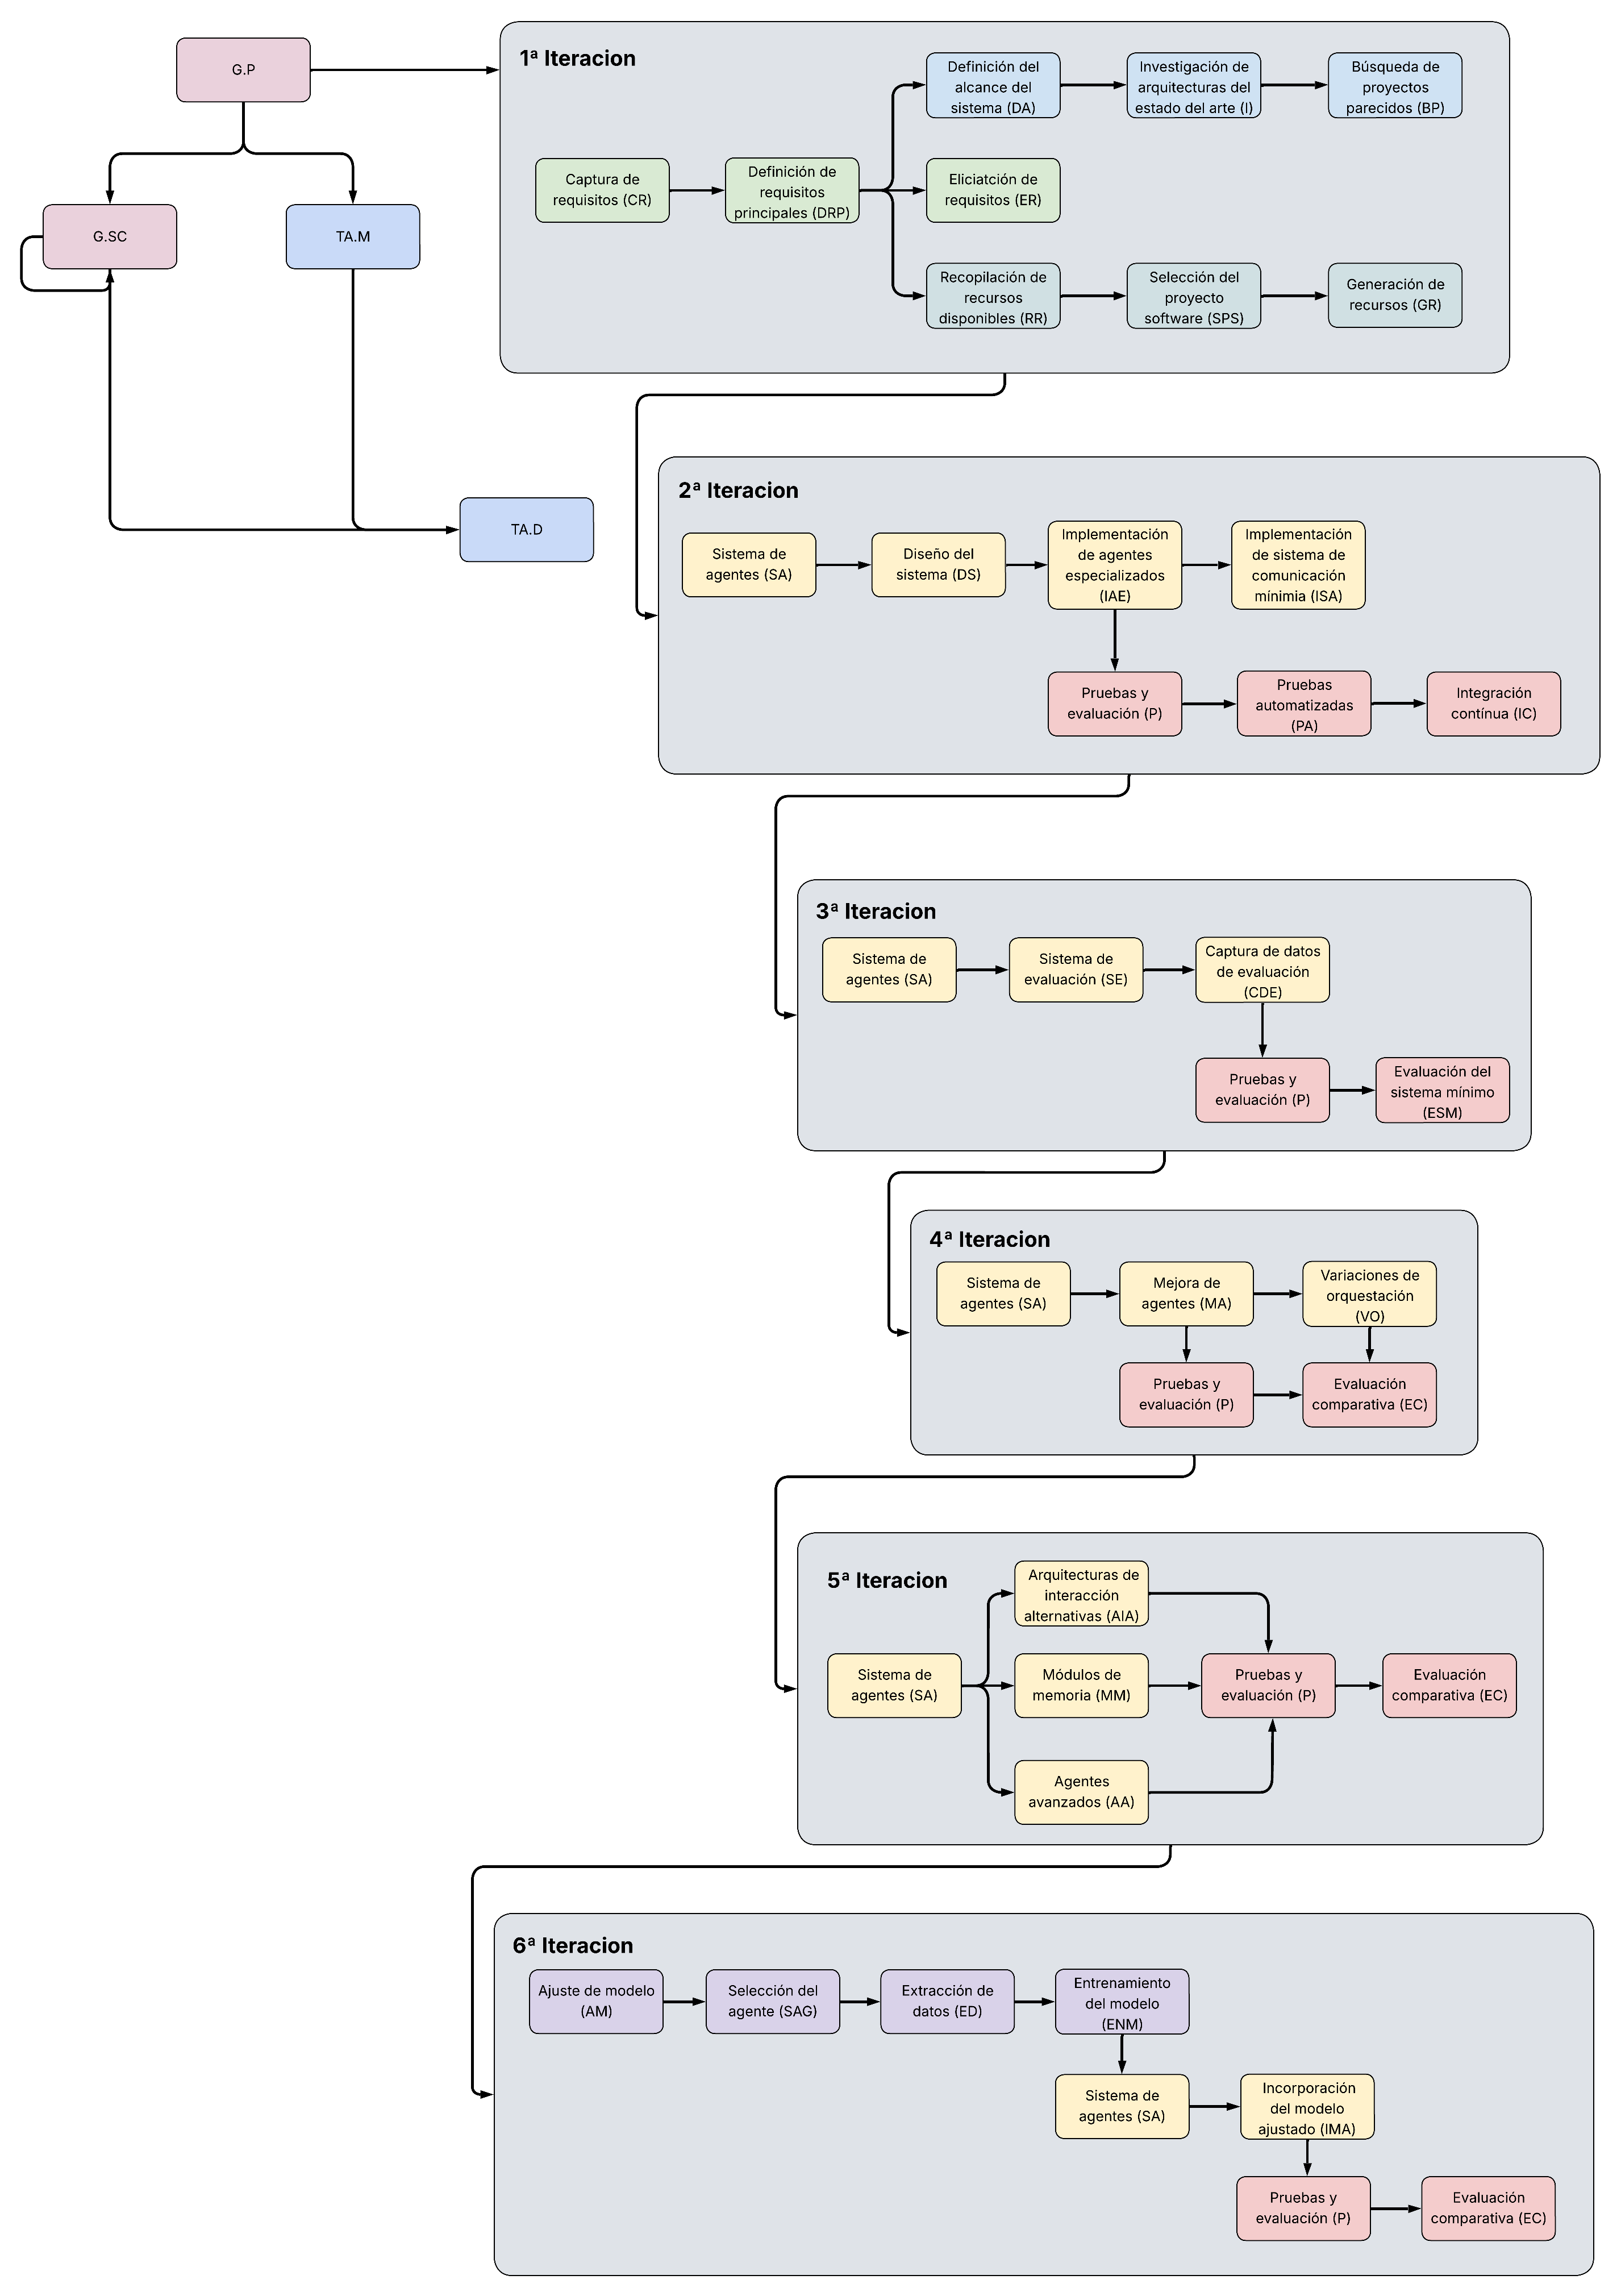
\includegraphics[scale=0.165]{figures/dependencias_2.png}%
  \caption{Dependencias entre tareas del proyecto}
  \label{fig:dependencias}
\end{figure}

El proyecto se inicia con una primera iteración centrada en la captura de requisitos, invertiendo un tiempo significativo en alinear los objetivos con las necesidades empresariales. Esta fase comprende la captura de requisitos (CR), la recopilación de recursos disponibles (RR) y la definición del alcance y requisitos del sistema de agentes (DA).

Las iteraciones intermedias desarrollan progresivamente el paquete Sistema de agentes (SA) mediante fases complementarias. La segunda iteración implementa su diseño conceptual, agentes especializados y un sistema de comunicación mínima. Posteriormente, en la tercera iteración, el sistema evoluciona incorporando mecanismos de evaluación y captura de datos. La cuarta iteración optimiza los agentes existentes y explora variaciones en la orquestación, mientras que la quinta implementa arquitecturas de interacción alternativas, módulos de memoria y agentes de procesamiento avanzado.

La sexta iteración introduce el paquete Ajuste de modelo (AM), que comprende la selección del agente candidato, extracción de datos y entrenamiento especializado. Simultáneamente, el paquete SA aborda actividades de integración del modelo ajustado en la arquitectura existente.

Transversalmente, se establecen los paquetes de Gestión (G), que abarca actividades de planificación y seguimiento mediante reuniones bisemanales, y Trabajo académico (TA), orientado a la elaboración de la memoria y preparación de la defensa.

Cabe destacar que a partir de la segunda iteración, cada fase incorpora el paquete de Pruebas y evaluación (P), destinado a verificar y analizar el rendimiento de los módulos implementados. Este paquete evoluciona progresivamente desde pruebas automatizadas básicas hasta evaluaciones comparativas que contrastan el rendimiento entre iteraciones sucesivas.

\subsection{Diagrama de Gantt}

La figura \ref{fig:gantt} muestra el diagrama de Gantt, donde se visualiza de manera aproximada la distribución temporal a cada paquete de trabajo durante el transcurso del proyecto. Los rombos negros señalan los hitos clave que se detallan en la sección \ref{sec:hitos}.

\definecolor{crcolor}{HTML}{6aa84f}
\definecolor{rrcolor}{HTML}{45818e}
\definecolor{dacolor}{HTML}{3d85c6}
\definecolor{sacolor}{HTML}{f1c232}
\definecolor{pcolor}{HTML}{cc0000}
\definecolor{amcolor}{HTML}{674ea7}
\definecolor{mdcolor}{HTML}{6d9eeb}

\begin{figure}[H]
  \noindent\hspace*{-1.75cm}
  \begin{ganttchart}[
    vgrid,
    hgrid,
    title label font=\bfseries,
    title height=1,
    bar height=0.6,
    x unit=0.15cm, 
    y unit title=0.7cm,
    y unit chart=0.6cm,
    time slot format=isodate,
    milestone/.style={
        shape=diamond,
        inner sep=2pt,
        draw=black,
        fill=black
    }
  ]{2025-02-25}{2025-06-30}
  
  \gantttitle{Proyecto 2025}{126} \\
  \gantttitle{Feb}{4}\gantttitle{Mar}{31}\gantttitle{Abr}{30}\gantttitle{May}{31}\gantttitle{Jun}{30} \\
  
  % Fila de hitos con rombos negros
  \ganttmilestone{}{2025-02-25} 
  \ganttmilestone{}{2025-03-20} 
  \ganttmilestone{}{2025-04-01} 
  \ganttmilestone{}{2025-04-15} 
  \ganttmilestone{}{2025-04-29} 
  \ganttmilestone{}{2025-05-13} 
  \ganttmilestone{}{2025-05-27} 
  \ganttmilestone{}{2025-06-14} \\
  
  % Barras regulares
  \ganttbar[bar/.style={fill=crcolor!70}]{PL}{2025-02-25}{2025-02-28} \\
  \ganttbar[bar/.style={fill=crcolor!70}]{SC}{2025-02-28}{2025-06-14} \\
  \ganttbar[bar/.style={fill=crcolor!70}]{CR}{2025-02-28}{2025-03-20} \\
  \ganttbar[bar/.style={fill=rrcolor!70}]{RR}{2025-02-28}{2025-03-20} \\
  \ganttbar[bar/.style={fill=dacolor!70}]{DA}{2025-02-28}{2025-03-20} \\
  \ganttbar[bar/.style={fill=sacolor!70}]{SA}{2025-03-20}{2025-05-27} \\
  \ganttbar[bar/.style={fill=pcolor!70}]{P}{2025-03-20}{2025-05-27} \\
  \ganttbar[bar/.style={fill=amcolor!70}]{AM}{2025-05-13}{2025-05-27} \\
  \ganttbar[bar/.style={fill=mdcolor!70}]{M}{2025-03-20}{2025-06-14} \\
  \ganttbar[bar/.style={fill=mdcolor!70}]{D}{2025-06-14}{2025-06-30} \\
  
  \end{ganttchart}
  \caption{Diagrama de Gantt del proyecto}
  \label{fig:gantt}
\end{figure}


\subsection{Hitos}\label{sec:hitos}

En la tabla \ref{tab:hitos} se detallan los hitos establecidos para el desarrollo del proyecto. La finalización de la fase de implementación ha sido programada para el 31 de mayo, tras lo cual se destinarán dos semanas íntegramente a la elaboración de la memoria hasta el 14 de junio, proporcionando así un margen de 8 días previos a la fecha límite de entrega. Este período de contingencia está planificado para abordar posibles contratiempos que pudieran surgir durante el transcurso del proyecto.

% CR(#d9ead3) / RR(#d0e0e3) / DA(#cfe2f3): 25/02 -> 20/03  
% SA(#fff2cc) / P(#f4cccc)  20/03 -> 27/05 
% AM(#d9d2e9) -> 13/05 -> 27/05
% M(#c9daf8): 20/03 -> 14/06/2025
% D(#c9daf8): 14/06 -> 30/06

\begin{table}[H]\centering
\begin{tabular}{|l|c|}
\hline
\multicolumn{1}{|c|}{\textbf{Hito}} & \multicolumn{1}{c|}{\textbf{Fecha}} \\
\hline
Inicio del proyecto & 25/02/2025 \\
\hline
Fin Iteración 1 & 20/03/2025 \\
\hline
Fin Iteración 2 & 01/04/2025 \\
\hline
Fin Iteración 3 & 15/04/2025 \\
\hline
Fin Iteración 4 & 29/04/2025 \\
\hline
Fin Iteración 5 & 13/05/2025 \\
\hline
Fin Iteración 6 & 27/05/2025 \\
\hline
Fin memoria & 14/06/2025 \\
\hline
Defensa del proyecto & Por determinar \\
\hline
\end{tabular}
\caption{Cronograma de Hitos del Proyecto}
\label{tab:hitos}
\end{table}

\section{Gestión del tiempo}
Se ha gestionado el tiempo disponible para el proyecto considerando el alcance definido para cumplir todos los objetivos del proyecto. 

\subsection{Estimación de cada tarea}
La estimación específica de cada tarea se puede ver en la tabla \ref{fig:horas}

\begin{figure}[h]
  \centering
  \adjustimage{width=1.3\textwidth,center}{figures/horas.png}
  \caption{Estimación horaria de cada tarea}
  \label{fig:horas}
\end{figure}

\section{Gestión de riesgos}

Debido al enfoque exploratorio del proyecto, la gestión de riesgos cobra especial importancia. Se han identificado los siguientes riesgos con su correspondiente plan de contingencia: 

\begin{itemize}
  \item\textbf{R1- Concurrencia exploratoria: }Dado que el proyecto está enfocado en tecnologías emergentes, existe la posibilidad de que durante el período de desarrollo emerjan iniciativas paralelas que aborden la misma problemática.  

Para abordar este riesgo, se realizará una previa investigación de soluciones existentes antes de implementar cada módulo del sistema, así como un análisis periódico que permita identificar mejoras inspiradas en avances externos.

\item\textbf{R2- Variabilidad del alcance: }Al ser un proyecto exploratorio, con un alcance inicialmente ambiguo, podría sufrir alteraciones no planificadas. Estos contratiempos podrían suponer un sobrecoste horario, lo que obligaría a replanificar el alcance para no sobrepasar ampliamente los recursos disponibles.

Para mitigar este riesgo, se implementará un seguimiento y control mediante reuniones quincenales que permitirán evaluar la correcta evolución de las actividades y, en caso necesario, adoptar medidas correctivas para garantizar la viabilidad del trabajo dentro de los plazos establecidos.


\item\textbf{R3- Dependencia de sistemas externos: }La implementación del proyecto depende significativamente de sistemas externos, tanto por los modelos de lenguaje accedidos a través de APIs como por los servicios proporcionados por los servidores MCP. Cualquier alteración o interrupción en estos servicios podría comprometer la funcionalidad del sistema implementado.

Para prevenir este riesgo, se diseñará un sistema con un manejo de excepciones robusto que garantice la continuidad operativa incluso cuando alguno de los módulos experimente fallos. Complementariamente, se adoptará una arquitectura de desarrollo modular que facilite la integración o desacoplamiento de componentes según las necesidades evolutivas del proyecto.

\item\textbf{R4- Filtrado de credenciales: }El acceso a recursos externos sobre el que se desarrolla el proyecto requiere de claves secretas. Es necesario considerar que existen algoritmos de rastreo automatizados que analizan plataformas públicas en busca de credenciales expuestas para su uso fraudulento. La publicación inadvertida de estas claves en entornos públicos podría ocasionar pérdidas económicas considerables o comprometer la seguridad del sistema corporativo.

Para contrarrestar este riesgo, se implementará una política de gestión de credenciales mediante variables de entorno, evitando su inclusión directa en el código fuente o su transferencia a plataformas en la nube. Adicionalmente, se mantendrán todos los repositorios y sistemas posibles en modo de visibilidad privada.

\item\textbf{R5- Pérdida de recursos: }El desarrollo del proyecto se fundamenta en múltiples recursos esenciales, incluyendo el código fuente del sistema, la documentación de requisitos, los diversos artefactos generados durante el proceso de desarrollo y la propia memoria académica. La pérdida de cualquiera de estos elementos debido a fallos técnicos o incidentes fortuitos podría ocasionar un retraso significativo.

Para mitigar este riesgo, se han implementado los sistemas de información descritos en la sección \ref{sec:sys_info} que garantizan el mantenimiento de copias de seguridad actualizadas diariamente en la nube. Mediante esta estrategia preventiva, cualquier eventualidad que afecte al dispositivo principal de desarrollo supondría, como máximo, la pérdida del trabajo correspondiente a una jornada.
\end{itemize}

\section{Gestión de Comunicaciones e Información}

\subsection{Sistema de información}\label{sec:sys_info}

La gestión de la información del proyecto se ha estructurado mediante los siguientes sistemas tecnológicos:
\begin{itemize}
\item \textbf{Repositorio GitHub para código fuente:} El código desarrollado será alojado en un repositorio privado de GitHub.
\item \textbf{Repositorio GitHub para documentación:} La memoria del proyecto, elaborada utilizando LaTeX en el entorno local del alumno, será sincronizada con un repositorio dedicado en GitHub.
\item \textbf{Almacenamiento en Google Drive:} Los diversos recursos y materiales auxiliares recopilados durante las fases de desarrollo serán almacenados en esta plataforma.
\end{itemize}
Esta estructura de gestión de la información aporta diversos beneficios al proyecto. Por un lado, facilita la supervisión continua por parte de los directores e implementa un control de versiones organizado que documenta la evolución del trabajo. Por otro lado, garantiza copias de seguridad actualizadas que protegen la integridad de los datos. Adicionalmente, asegura la accesibilidad para todos los interesados.


\subsection{Sistema de comunicación}
La comunicación eficaz entre alumno, director empresarial y directores académicos resulta imprescindible para el correcto seguimiento y control del proyecto. Las herramientas a utilizar son:
\begin{itemize}
\item\textbf{Correo electrónico: }Canal principal para consultas con los directores del proyecto y comunicación formal con otros miembros de la empresa.
\item\textbf{Google Meet: }Plataforma destinada a la realización de reuniones telemáticas entre los participantes.
\item\textbf{Google Chat: }Herramienta complementaria para resolución de consultas rápidas con el director empresarial.
\end{itemize}

\section{Herramientas disponibles}
Para el desarrollo del proyecto se dispone de varias herramientas que facilitan su implementación y gestión eficiente:
\begin{itemize}
\item\textbf{IDE PyCharm: }Se usará la versión Professional del entorno de desarrollo PyCharm\footnote{PyCharm: \url{https://www.jetbrains.com/es-es/pycharm/}}, obtenida a través del paquete educativo de GitHub, que proporciona herramientas especializadas para el desarrollo en Python.
\item\textbf{Asistencia de herramientas de inteligencia artificial: }Se dispone de herramientas de asistencia basadas en inteligencia artificial como GitHub Copilot y una suscripción al modelo Claude, que optimizan las tareas de programación, el procesamiento documental y la redacción de la presente memoria.
\item\textbf{Claves de acceso a modelos: }La empresa LKS NEXT ha facilitado las credenciales de acceso necesarias para la integración y ejecución de los diferentes modelos LLM utilizados en el proyecto.
\item\textbf{Plataformas de computación en la nube: }Se dispone de acceso a infraestructuras de computación en la nube con unidades de procesamiento gráfico (GPU) dedicadas para el entrenamiento e inferencia del modelo ajustado.
\end{itemize}












